% ============================================================================
% CSCE 763: Digital Image Processing - Homework 3
% ============================================================================

\documentclass[12pt]{article}

% ============================================================================
% PACKAGE IMPORTS
% ============================================================================
\usepackage{amsmath}
\usepackage{graphicx}
\usepackage{amssymb}
\usepackage{tikz}
\usepackage[margin=1in]{geometry}
\usepackage{setspace}
\usepackage{xcolor}
\usepackage{enumitem}
\usepackage{tcolorbox}
\usepackage{fancyhdr}
\usepackage{booktabs}
\usepackage{array}
\usepackage{colortbl}
\usepackage{float}

% ============================================================================
% HEADER AND FOOTER SETUP
% ============================================================================
\pagestyle{fancy}
\setlength{\headheight}{14.5pt}
\fancyhf{}

\fancyhead[L]{Page \thepage}
\fancyhead[C]{CSCE 763}
\fancyhead[R]{JC Vaught}

\renewcommand{\headrulewidth}{0pt}

% ============================================================================
% TIKZ LIBRARIES
% ============================================================================
\usetikzlibrary{shapes.geometric, arrows.meta, positioning, patterns}

% --- USC Brand Colors ---
\definecolor{USC_Garnet}{HTML}{73000A}
\definecolor{USC_Sandstorm}{HTML}{FFF2E3}
\definecolor{USC_Black90}{HTML}{363636}
\definecolor{USC_Black70}{HTML}{5C5C5C}
\definecolor{USC_Black50}{HTML}{A2A2A2}
\definecolor{USC_Black10}{HTML}{ECECEC}
\definecolor{USC_Honeycomb}{HTML}{65780B}
\definecolor{USC_Atlantic}{HTML}{466A9F}
\definecolor{USC_Congaree}{HTML}{1F414D}
\definecolor{USC_Rose}{HTML}{CC2E40}
\definecolor{outputbg}{RGB}{245,245,245}
\definecolor{tealfill}{HTML}{00B8A9}
\definecolor{teallight}{HTML}{D4F0ED}
\definecolor{lightblue}{HTML}{D6EAF8}

% ============================================================================
% CUSTOM COLORED BOXES
% ============================================================================
\newtcolorbox{stepbox}[1][Step]{
  colback=white,
  colframe=USC_Garnet,
  fonttitle=\bfseries,
  title=#1,
  sharp corners,
  colbacktitle=USC_Garnet,
  coltitle=white,
}

\newtcolorbox{resultsbox}{
  colback=white,
  colframe=USC_Honeycomb,
  fonttitle=\bfseries,
  title=Results,
  sharp corners,
  colbacktitle=USC_Honeycomb,
  coltitle=white,
}

% ============================================================================
% CUSTOM QUESTION AND PART COMMANDS
% ============================================================================
\newcommand{\question}[1]{%
  \clearpage
  \vspace{0.5cm}
  {\noindent\normalsize \textbf{#1}}
  \vspace{0.2cm}
  \hrule
  \vspace{0.1cm}
  \hrule
  \vspace{0.3cm}
}

\newcommand{\questionpart}[1]{%
  \clearpage
  \vspace{0.5cm}
  {\noindent\normalsize \textbf{#1}}
  \vspace{0.2cm}
  \hrule
  \vspace{0.1cm}
  \hrule
  \vspace{0.3cm}
}

% Graphics path
\graphicspath{{figures/}}

% ============================================================================
% DOCUMENT INFORMATION
% ============================================================================

\title{CSCE 763: Digital Image Processing \\ Homework \#3}
\author{Instructor: Spring 2026 \\ University of South Carolina \\ \textit{Solutions by: JC Vaught}}
\date{Due: 1:15 pm EST, Tuesday, Feb 17}

% ============================================================================
% BEGIN DOCUMENT
% ============================================================================

\begin{document}

\maketitle
\setlength{\parindent}{0pt}

\setlist[enumerate,1]{label=\arabic*.}
\setlist[enumerate,2]{label=(\alph*)}

% ============================================================================
% TABLE OF CONTENTS
% ============================================================================

\begin{center}
\begin{tcolorbox}[colback=white, colframe=gray!50!black, colbacktitle=gray!20!white,
                  coltitle=black, sharp corners, boxrule=1pt,
                  title=\Large\bfseries Table of Contents]
\begin{tabular}{p{0.82\textwidth}r}
\textbf{Problem 1: Histogram and Blurring (20 pts)} \dotfill & \textbf{\pageref{quest:1}} \\[0.3em]
\textbf{Problem 2: Spatial Filtering (20 pts)} \dotfill & \textbf{\pageref{quest:2}} \\[0.3em]
\textbf{Problem 3: Averaging Mask and Bar Merging (20 pts)} \dotfill & \textbf{\pageref{quest:3}} \\[0.3em]
\textbf{Problem 4: Averaging and Laplacian Order (20 pts)} \dotfill & \textbf{\pageref{quest:4}} \\[0.3em]
\textbf{Problem 5: Convolution Filtering (20 pts)} \dotfill & \textbf{\pageref{quest:5}} \\
\end{tabular}
\vspace{0.2cm}
\end{tcolorbox}
\end{center}

\vspace{0.5cm}

% ============================================================================
% PROBLEM 1: Histogram and Blurring
% ============================================================================

\question{Problem 1: Histogram and Blurring (20 pts)}\label{quest:1}

Two $N \times N$ images shown below are quite different, but their histograms are the same. Suppose that each image is blurred with a $3 \times 3$ averaging mask. Please ignore the low quality of the images. You can assume all the black regions have a uniform intensity of 0, and the white regions have a uniform intensity of 255.

\begin{enumerate}[label=(\alph*)]
\item Would the histogram of the blurred images still be equal? Explain.
\item If your answer is no, sketch the two histograms.
\item \textbf{Bonus question:} Discuss how the histogram of the blurred Figure~1(b) is affected by different image size $N$. (5 pts)
\end{enumerate}

\vspace{0.5cm}

\begin{center}
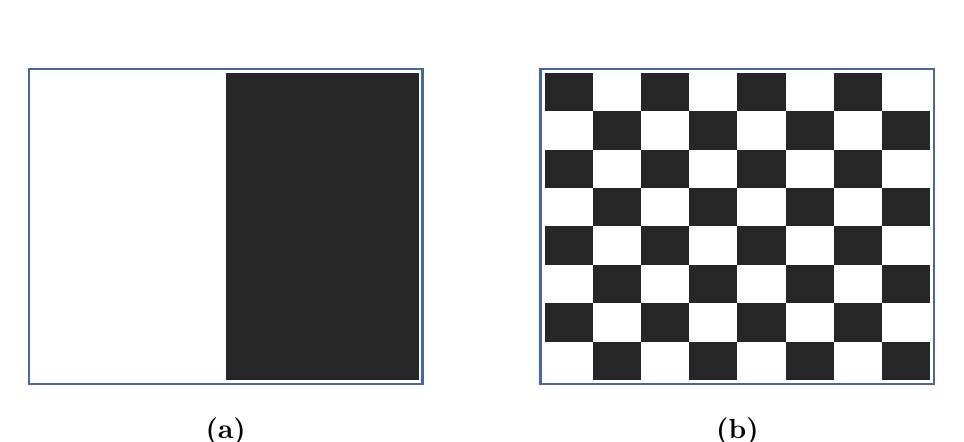
\begin{tikzpicture}
  % Figure 1(a): White left, black right
  \draw[thick, USC_Atlantic] (0,0) rectangle (5,4);
  \fill[white] (0.05,0.05) rectangle (2.5,3.95);
  \fill[black!85] (2.5,0.05) rectangle (4.95,3.95);
  \node[below] at (2.5,-0.3) {\textbf{(a)}};

  % Figure 1(b): Chessboard
  \begin{scope}[shift={(6.5,0)}]
    \draw[thick, USC_Atlantic] (0,0) rectangle (5,4);
    \foreach \i in {0,...,7} {
      \foreach \j in {0,...,7} {
        \pgfmathtruncatemacro{\checkcolor}{mod(\i+\j,2)}
        \ifnum\checkcolor=0
          \fill[white] ({0.05+\i*0.6125}, {0.05+\j*0.4875}) rectangle ({0.05+\i*0.6125+0.6125}, {0.05+\j*0.4875+0.4875});
        \else
          \fill[black!85] ({0.05+\i*0.6125}, {0.05+\j*0.4875}) rectangle ({0.05+\i*0.6125+0.6125}, {0.05+\j*0.4875+0.4875});
        \fi
      }
    }
    \node[below] at (2.5,-0.3) {\textbf{(b)}};
  \end{scope}
\end{tikzpicture}
\end{center}

\vspace{0.3cm}
\begin{center}
\textbf{Figure 1.} (a) An image with white intensities on left and black intensities on the right. (b) A chessboard image.
\end{center}


% ============================================================================
% PROBLEM 2: Spatial Filtering
% ============================================================================

\question{Problem 2: Spatial Filtering (20 pts)}\label{quest:2}

Consider spatial filtering.

\begin{enumerate}[label=(\alph*)]
\item Suppose that you filter an image $f(x,y)$, with a spatial filter mask $w(x,y)$, using convolution, as defined in Eq.~(3.4-2), where the mask is smaller than the image in both spatial directions. Show the important property that, if the coefficients of the mask sum to zero, then the sum of all the elements in the resulting convolution array (filtered image) will be zero also (you may ignore computational inaccuracies). Also, you may assume that the border of the image has been padded with the appropriate number of zeros. (10 pts)
\begin{align}
w(x,y) \otimes f(x,y) = \sum_{s=-a}^{a} \sum_{t=-b}^{b} w(s,t)\, f(x-s, y-t) \tag{3.4-2}
\end{align}

\item Would the result to (a) be the same if the filtering is implemented using correlation, as defined in Eq.~(3.4-1)? (10 pts)
\begin{align}
w(x,y) \odot f(x,y) = \sum_{s=-a}^{a} \sum_{t=-b}^{b} w(s,t)\, f(x+s, y+t) \tag{3.4-1}
\end{align}
\end{enumerate}


% ============================================================================
% PROBLEM 3: Averaging Mask and Bar Merging
% ============================================================================

\question{Problem 3: Averaging Mask and Bar Merging (20 pts)}\label{quest:3}

The three images shown were blurred using square averaging masks of sizes $n=23$, 25, and 45, respectively. The vertical bars on the left lower part of Figure~3(a) and (c) are blurred, but a clear separation exists between them. However, the bars have merged in image Figure~3(b), in spite of the fact that the mask that produced this image is significantly smaller than the mask that produced image Figure~3(c). Explain the reason for this. The vertical bars are 5 pixels wide, 100 pixels high, and their separation is 20 pixels. (Hints: you can simplify the problem by considering a single scan line through the bars in the image.)

\vspace{0.5cm}

\begin{center}
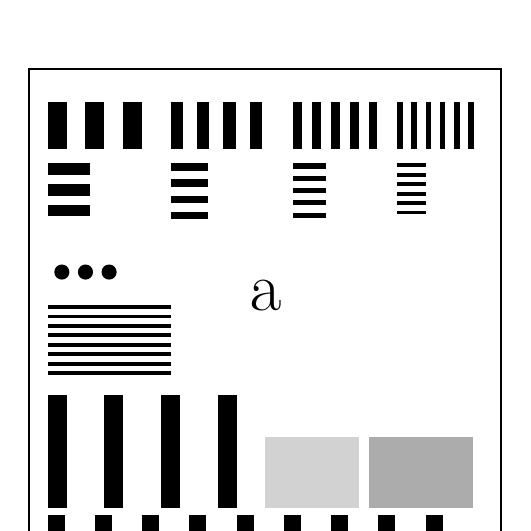
\begin{tikzpicture}[scale=1.2]
  \fill[white] (0,0) rectangle (5,5);
  \draw[thick] (0,0) rectangle (5,5);

  % === TOP SECTION: 4 groups of vertical bars + horizontal bars below ===
  % Group 1 (largest bars)
  \foreach \i in {0,...,2} {
    \fill[black] (0.2+\i*0.4, 4.65) rectangle (0.2+\i*0.4+0.2, 4.15);
  }
  \foreach \i in {0,...,2} {
    \fill[black] (0.2, 4.0-\i*0.22) rectangle (0.65, 4.0-\i*0.22-0.12);
  }

  % Group 2
  \foreach \i in {0,...,3} {
    \fill[black] (1.5+\i*0.28, 4.65) rectangle (1.5+\i*0.28+0.13, 4.15);
  }
  \foreach \i in {0,...,3} {
    \fill[black] (1.5, 4.0-\i*0.17) rectangle (1.9, 4.0-\i*0.17-0.08);
  }

  % Group 3
  \foreach \i in {0,...,4} {
    \fill[black] (2.8+\i*0.2, 4.65) rectangle (2.8+\i*0.2+0.09, 4.15);
  }
  \foreach \i in {0,...,4} {
    \fill[black] (2.8, 4.0-\i*0.13) rectangle (3.15, 4.0-\i*0.13-0.055);
  }

  % Group 4 (smallest bars)
  \foreach \i in {0,...,5} {
    \fill[black] (3.9+\i*0.15, 4.65) rectangle (3.9+\i*0.15+0.06, 4.15);
  }
  \foreach \i in {0,...,5} {
    \fill[black] (3.9, 4.0-\i*0.1) rectangle (4.2, 4.0-\i*0.1-0.04);
  }

  % === MIDDLE SECTION ===
  % Three dots
  \foreach \i in {0,...,2} {
    \fill[black] (0.35+\i*0.25, 2.85) circle (0.08);
  }

  % Large "a"
  \node[font=\fontsize{40}{40}\selectfont, anchor=center] at (2.5, 2.6) {a};

  % Horizontal ruled lines (left side, below dots)
  \foreach \i in {0,...,7} {
    \fill[black] (0.2, 2.5-\i*0.1) rectangle (1.5, 2.5-\i*0.1-0.04);
  }

  % === BOTTOM SECTION ===
  % Vertical bars: 5px wide, 20px gap (scaled: bar=0.2cm, gap=0.8cm period)
  \foreach \i in {0,...,3} {
    \fill[black] (0.2+\i*0.6, 0.35) rectangle (0.2+\i*0.6+0.2, 1.55);
  }

  % Gray patches (lower right)
  \fill[gray!35] (2.5, 0.35) rectangle (3.5, 1.1);
  \fill[gray!65] (3.6, 0.35) rectangle (4.7, 1.1);

  % Bottom row: small squares
  \foreach \i in {0,...,8} {
    \fill[black] (0.2+\i*0.5, 0.1) rectangle (0.2+\i*0.5+0.18, 0.28);
  }

  \draw[thick] (0,0) rectangle (5,5);
\end{tikzpicture}
\end{center}

\vspace{0.3cm}
\begin{center}
\textbf{Figure 2.} Original resolution test chart. The vertical bars (bottom left) are 5 pixels wide with 20 pixels of separation.
\end{center}

\vspace{0.5cm}

% === Three blurred versions ===
\begin{center}
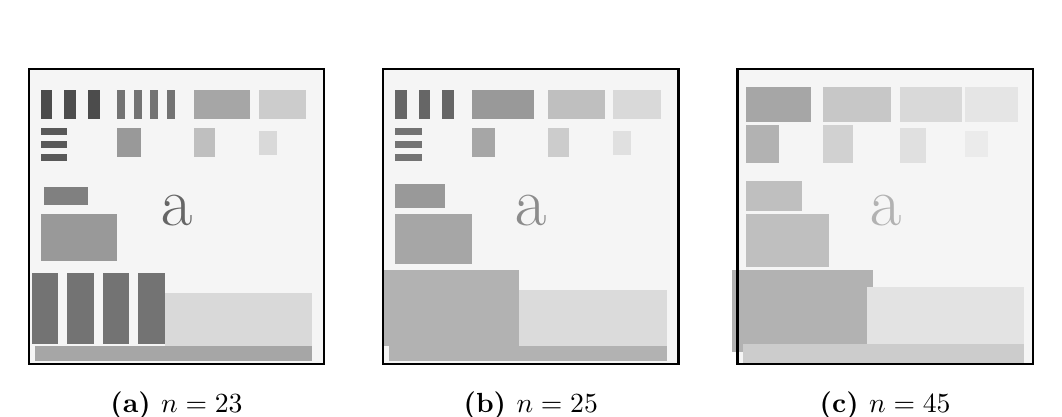
\begin{tikzpicture}[scale=0.75]

% ========== (a) n=23: mild blur, bars still separated ==========
\begin{scope}[shift={(0,0)}]
  \fill[gray!8] (0,0) rectangle (5,5);
  \draw[thick] (0,0) rectangle (5,5);

  % Top bars: group 1 blurred but visible
  \foreach \i in {0,...,2} {
    \fill[black!70] (0.2+\i*0.4, 4.65) rectangle (0.2+\i*0.4+0.2, 4.15);
  }
  % Group 2 blurred
  \foreach \i in {0,...,3} {
    \fill[black!55] (1.5+\i*0.28, 4.65) rectangle (1.5+\i*0.28+0.13, 4.15);
  }
  % Group 3 heavily blurred
  \fill[black!35] (2.8, 4.65) rectangle (3.75, 4.15);
  % Group 4 merged
  \fill[black!20] (3.9, 4.65) rectangle (4.7, 4.15);

  % Horizontal bar groups blurred
  \foreach \i in {0,...,2} {
    \fill[black!65] (0.2, 4.0-\i*0.22) rectangle (0.65, 4.0-\i*0.22-0.12);
  }
  \fill[black!40] (1.5, 3.5) rectangle (1.9, 4.0);
  \fill[black!25] (2.8, 3.5) rectangle (3.15, 4.0);
  \fill[black!15] (3.9, 3.55) rectangle (4.2, 3.95);

  % Dots blurred
  \fill[black!50] (0.25, 2.7) rectangle (1.0, 3.0);

  % "a" blurred
  \node[font=\fontsize{36}{36}\selectfont, text=black!60, anchor=center] at (2.5, 2.6) {a};

  % Horizontal lines: merged into gray band
  \fill[black!40] (0.2, 1.75) rectangle (1.5, 2.55);

  % Vertical bars: STILL SEPARATED (key for n=23)
  \foreach \i in {0,...,3} {
    \fill[black!55] ({0.05+\i*0.6}, 0.35) rectangle ({0.05+\i*0.6+0.45}, 1.55);
  }

  % Gray patches: blurred together
  \fill[gray!30] (2.3, 0.25) rectangle (4.8, 1.2);

  % Bottom squares: merged into bar
  \fill[black!35] (0.1, 0.05) rectangle (4.8, 0.3);

  \draw[thick] (0,0) rectangle (5,5);
  \node[below, font=\bfseries] at (2.5,-0.3) {(a) $n=23$};
\end{scope}

% ========== (b) n=25: bars MERGED (period = mask size) ==========
\begin{scope}[shift={(6,0)}]
  \fill[gray!8] (0,0) rectangle (5,5);
  \draw[thick] (0,0) rectangle (5,5);

  % Top bars: group 1 blurred
  \foreach \i in {0,...,2} {
    \fill[black!60] (0.2+\i*0.4, 4.65) rectangle (0.2+\i*0.4+0.2, 4.15);
  }
  % Groups 2-4 merged
  \fill[black!40] (1.5, 4.15) rectangle (2.55, 4.65);
  \fill[black!25] (2.8, 4.15) rectangle (3.75, 4.65);
  \fill[black!15] (3.9, 4.15) rectangle (4.7, 4.65);

  % Horizontal bars merged
  \foreach \i in {0,...,2} {
    \fill[black!55] (0.2, 4.0-\i*0.22) rectangle (0.65, 4.0-\i*0.22-0.12);
  }
  \fill[black!35] (1.5, 3.5) rectangle (1.9, 4.0);
  \fill[black!20] (2.8, 3.5) rectangle (3.15, 4.0);
  \fill[black!12] (3.9, 3.55) rectangle (4.2, 3.95);

  % Dots fully blurred
  \fill[black!40] (0.2, 2.65) rectangle (1.05, 3.05);

  % "a" more blurred
  \node[font=\fontsize{36}{36}\selectfont, text=black!45, anchor=center] at (2.5, 2.6) {a};

  % Horizontal lines: fully merged
  \fill[black!35] (0.2, 1.7) rectangle (1.5, 2.55);

  % Vertical bars: MERGED into uniform gray (key for n=25)
  \fill[black!30] (0.0, 0.3) rectangle (2.3, 1.6);

  % Gray patches
  \fill[gray!28] (2.3, 0.2) rectangle (4.8, 1.25);

  % Bottom squares: merged
  \fill[black!30] (0.1, 0.05) rectangle (4.8, 0.3);

  \draw[thick] (0,0) rectangle (5,5);
  \node[below, font=\bfseries] at (2.5,-0.3) {(b) $n=25$};
\end{scope}

% ========== (c) n=45: heavy blur, but bars still separated ==========
\begin{scope}[shift={(12,0)}]
  \fill[gray!8] (0,0) rectangle (5,5);
  \draw[thick] (0,0) rectangle (5,5);

  % Top bars: all heavily blurred/merged
  \fill[black!35] (0.15, 4.1) rectangle (1.25, 4.7);
  \fill[black!22] (1.45, 4.1) rectangle (2.6, 4.7);
  \fill[black!15] (2.75, 4.1) rectangle (3.8, 4.7);
  \fill[black!10] (3.85, 4.1) rectangle (4.75, 4.7);

  % Horizontal bars: all merged
  \fill[black!30] (0.15, 3.4) rectangle (0.7, 4.05);
  \fill[black!18] (1.45, 3.4) rectangle (1.95, 4.05);
  \fill[black!12] (2.75, 3.4) rectangle (3.2, 4.0);
  \fill[black!8] (3.85, 3.5) rectangle (4.25, 3.95);

  % Dots: gone
  \fill[black!25] (0.15, 2.6) rectangle (1.1, 3.1);

  % "a" very blurred
  \node[font=\fontsize{36}{36}\selectfont, text=black!30, anchor=center] at (2.5, 2.6) {a};

  % Horizontal lines: fully merged
  \fill[black!25] (0.15, 1.65) rectangle (1.55, 2.55);

  % Vertical bars: STILL SEPARATED despite heavy blur (key for n=45)
  \foreach \i in {0,...,3} {
    \fill[black!30] ({-0.1+\i*0.6}, 0.2) rectangle ({-0.1+\i*0.6+0.6}, 1.6);
  }

  % Gray patches
  \fill[gray!22] (2.2, 0.15) rectangle (4.85, 1.3);

  % Bottom: merged
  \fill[black!20] (0.1, 0.0) rectangle (4.85, 0.35);

  \draw[thick] (0,0) rectangle (5,5);
  \node[below, font=\bfseries] at (2.5,-0.3) {(c) $n=45$};
\end{scope}

\end{tikzpicture}
\end{center}

\vspace{0.3cm}
\begin{center}
\textbf{Figure 3.} Three images smoothed by averaging using different filters. Note the vertical bars merge in~(b) despite the smaller mask size.
\end{center}


% ============================================================================
% PROBLEM 4: Averaging and Laplacian Order
% ============================================================================

\question{Problem 4: Averaging and Laplacian Order (20 pts)}\label{quest:4}

In a given application an averaging mask is applied to input images to reduce noise, and then a Laplacian mask is applied to enhance small details. Would the result be the same if the order of these operations were reversed?


% ============================================================================
% PROBLEM 5: Convolution Filtering
% ============================================================================

\question{Problem 5: Convolution Filtering (20 pts)}\label{quest:5}

Given the following $3 \times 3$ filter, perform the image filtering using \textbf{convolution}. Give the \textbf{FULL} filtering result for each filtering process. (Hint: you need to assume an appropriate zero mapping.)
%
\[
w = \begin{bmatrix} -1 & 0 & -1 \\ 0 & 2 & 0 \\ 1 & 0 & 1 \end{bmatrix}
\]
%
\begin{enumerate}[label=(\alph*)]
\item a $2 \times 2$ image as shown in Figure~4(a) \hfill (10 pts)
\item a $3 \times 3$ image as shown in Figure~4(b) \hfill (10 pts)
\end{enumerate}

\vspace{0.5cm}

\begin{center}
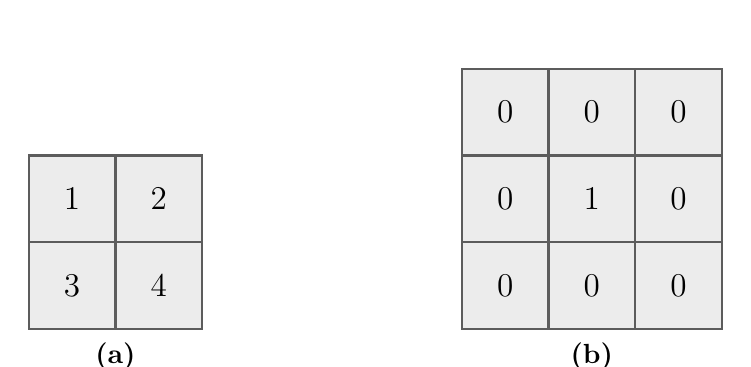
\begin{tikzpicture}[
  imgcell/.style={minimum size=1.1cm, draw=USC_Black70, thick, fill=USC_Black10, font=\large\bfseries},
  gridcell/.style={minimum size=1.1cm, draw=USC_Black70, thick, fill=USC_Black10, font=\large\bfseries},
]

% --- (a) 2x2 image ---
\node[imgcell] at (0, 1.1) {$1$};
\node[imgcell] at (1.1, 1.1) {$2$};
\node[imgcell] at (0, 0) {$3$};
\node[imgcell] at (1.1, 0) {$4$};
\node[font=\bfseries] at (0.55, -0.9) {(a)};

% --- (b) 3x3 identity image ---
\foreach \val/\col/\row in {
  0/0/2, 0/1/2, 0/2/2,
  0/0/1, 1/1/1, 0/2/1,
  0/0/0, 0/1/0, 0/2/0}
{
  \node[gridcell] at (5.5+\col*1.1, \row*1.1) {$\val$};
}
\node[font=\bfseries] at (6.6, -0.9) {(b)};

\end{tikzpicture}
\end{center}

\vspace{0.3cm}
\begin{center}
\textbf{Figure 4.}
\end{center}


% ============================================================================
% END OF DOCUMENT
% ============================================================================

\end{document}
